\section{Esecuzione}

Avendo a disposizione due tipi di pompe da vuoto, abbiamo deciso di ricavare la velocità di pompaggio per entrambi gli strumenti.

Poiché la pompa turbomolecolare ha bisogno di una decina di minuti per fermarsi abbiamo cominciato le misure con la pompa rotativa. Qundi, per calcolarne la velocità di pompaggio ci siamo mossi come segue:

\begin{itemize}
	\item{abbiamo isolato la pompa turbomolecolare;}
	\item{grazie al baypass abbiamo svuotato la camera da vuoto fino alla pressione limite della pompa rotativa, cioè una pressione di qualche Pascal;}
	\item{successivamente abbiamo prodotto mediante l'utilizzo della valvola a spillo un flusso costante di gas all'interno della camera da vuoto. Questo e stato possibile girando un numero opportuno di vote la vite micrometrica della valvola;}
	\item{quindi grazie al sistema di acquisiziione dati abbiamo registrato l'andamento della pressione interna alla camera in funzione del tempo. I dati sono stati presi finchè la curva non ha assunto una configurazine asintotica, ovvero fino a che la pressione in camera non si è stabilizzata attorno ad un valore costante;}
	\item{una volta che la pressione in camera si è stabilizzata, abbiamo svitato la vite micrometrica della valvola a spillo di un ulteriore giro e abbiamo registrato la variazione della pressione interna della camera in funzone del tempo;}
	\item{abbiamo ripetuto quest'ultimo passaggio fino a che la vite micrometrica non è stata svitata di 9 tornate;} %qualche dubbio
\end{itemize}

Per calcolare la velocità di pompaggio della pompa turbomolecolare abbiamo seguito lo stesso procedimento descritto sopra fatta eccezione che in questo caso il baypass non era attivo, in quanto il vuoto in camera è effettuato mediante la pompa turbolecolare.
Un'altra differenza tra le due procedure risiede nel numero di giri della vite micrometrica che si sono fatti. Per la pompa rotativa siamo partiti da quattro giri della valvola a spillo fino ad arrivare al nono giro. Per la pompa turbomolecolare invece siamo partiti con un flusso di gas equivalnte ad un giro di valvola a spillo e siamo arrivati fino a sei giri di valvola. Facciamo notare che per la pompa turbomolecolare non è stato possibile fare ulteriori misure con un numero più elevato di giri in quanto la pressione in camera sarebbe risultata troppo elevata per il corretto funzionamento della pompa turbomolecolare, che lavora correttamnte in regime molecolare ovvero a pressioni inferiori a qualche Pascal.
Infine è doveroso sottolineare che per misurare la pressione in camera, quando era in azione la pompa turbomolecolare, non ci siamo più potuti avvalere del sistema di aquisizione dati connesso ai vacuometri Pirani, ma abbiamo douto utilizzare il vacuometro a catodo freddo Penning. Quindi la lettura della pressione è stata presa una volta che questa sembrava essersi stabilizzata e quindi non vi erano repentine variazioni della misura.  

\begin{figure}[b!]
	\centering
		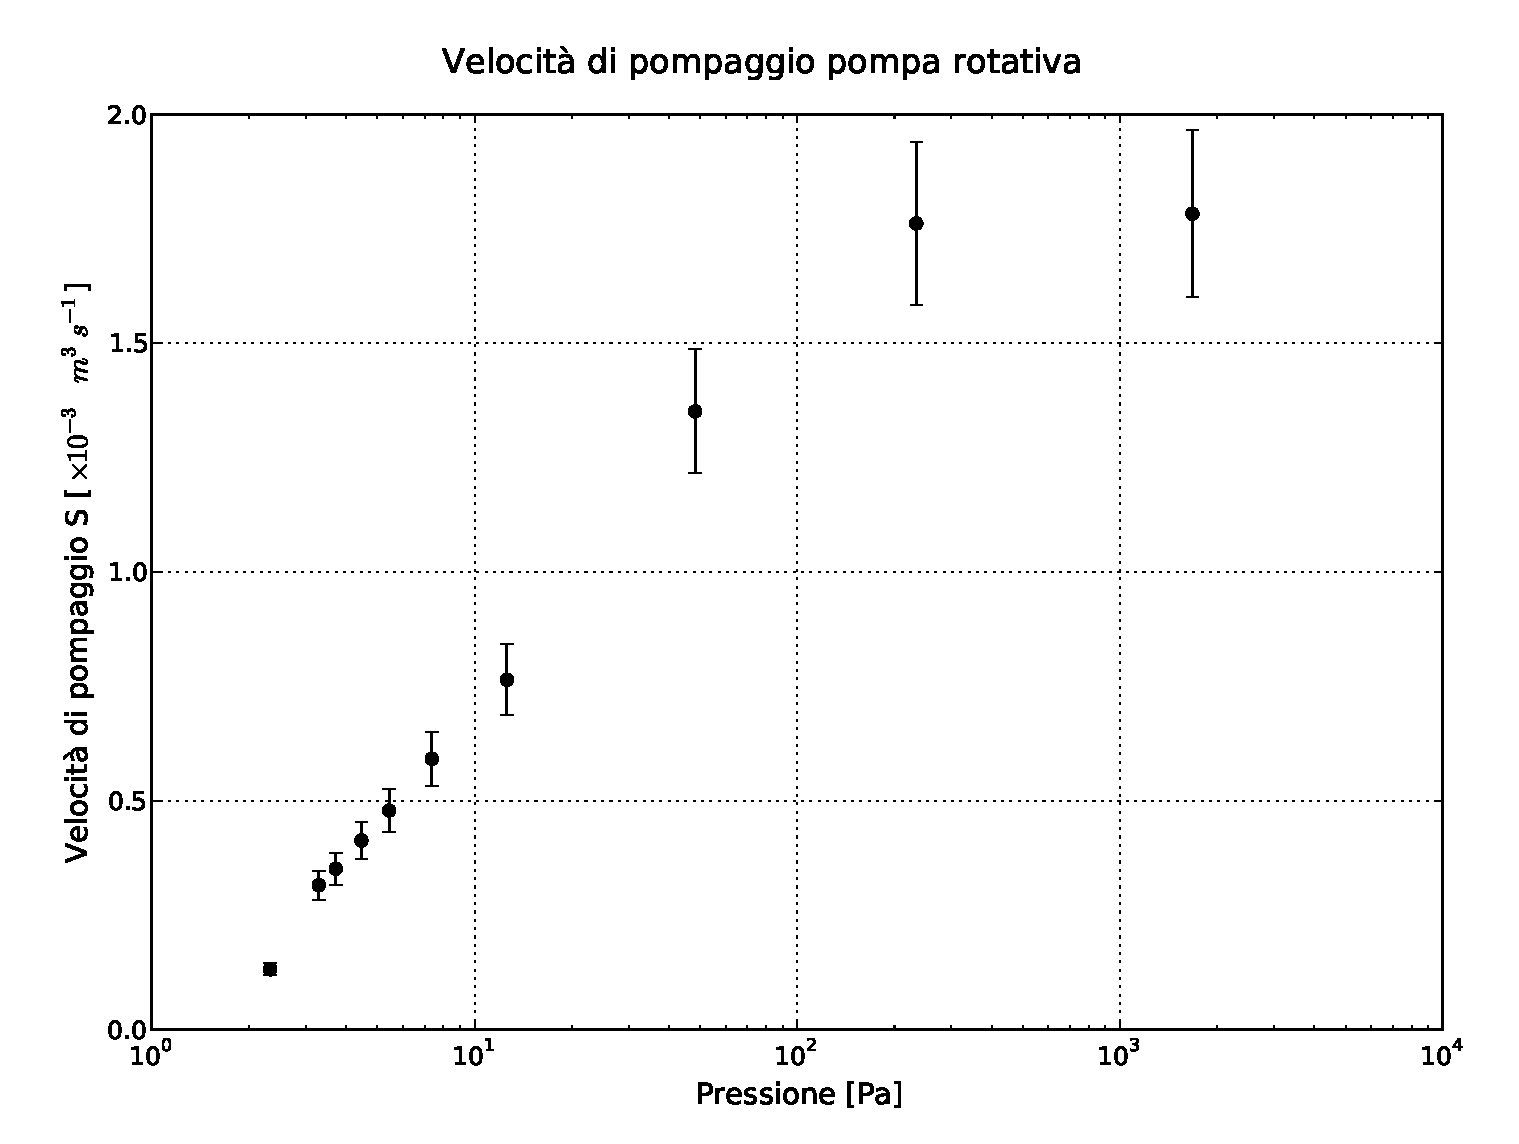
\includegraphics[width = 15cm]{rotativa.pdf}
		\label{fig:rotativa}
	\caption{Il grafico mostra i valori elaborati della velocità di pompaggio della pompa rotativa in funzione della pressione limite raggiunta in camera. L'asse delle ascisse ha scala logaritmica mentre l'asse delle ordinate ha scala lineare.}
\end{figure}

\section{Analisi dati}

Le condizioni ambientali presenti durante lo svolgimento di questa sessione di laboratorio sono le seguenti: tra le ore 14:00 e le 18:00 la temperatura e passata da 25$^\circ$ C a 27$^\circ$ C mentre la pressione atmosferica è rimasta stabile attorno ad un valore di circa $9.84\,\,10^4\, Pa$

Grazie all'esperienza di laboratorio precedente durante la quale abbiamo tarato la valvola a spillo noi conosciamo il flusso di gas in ingresso alla camera da vuoto in funzione del numero di giri apportati alla vite micrometrica della valvola.
Pertanto per ricavare la velocità di pompaggio delle nostre pompe ci avvaliamo della seguente relazione:

\begin{equation}
	S \,=\, \frac{Q}{P}
\end{equation}
%
dove $S$ rappresenta la velocità di pompaggio della pompa in esame, $Q$ il flusso di gas in entrata nella camera da vuoto e $P$ rappresenta il valore della pressione una volta raggiunto l'andamento asintotico sopracitato. 
%
%
%
%
Infine abbiamo deciso di confrontare i valori relativi alle velocità di pompaggio da noi ottenuti con quelli forniteci dai costruttori. I dati forniti dalle case costruttrici sono i seguenti:
%
%

Come si può notare, i valori da noi trovati risultano essere inferiori, a volte anche in modo significativo, rispetto alle velocità di pompaggio indicate sul manuale dello strumento.
Tra i motivi che possono incidere su queste discrepanze fra i valori sperimentali e quelli teorici abbiamo ipotizzato che i più rilevanti siano:

\begin{itemize}
	\item{l'usura della pompa stessa che porta ad una minore efficienza;}
	\item{i valori forniti dal costruttore si riferiscono alla velocità di pompaggio alla bocca della pompa e non tengono conto della conduttanza delle canalizzazioni tra i vari componenti dell'impianto da vuoto. Tale differenza è particolarmente evidente soprattutto per la pompa rotativa. Infatti questa non era collegata direttamente alla camera da vuoto come lo era la pompa turbomolecolare, ma tramite un tubo di circa un metro di lunghezza;}%stimiamo la conduttanza???
\end{itemize}

\begin{table}
    \begin{tabular}{l c c c c c c}
        \toprule
        Nr. giri &
        $Q  [\si{\Pa\cubic\meter\per\second}]$ & $\sigma (Q) [\si{\Pa\cubic\meter\per\second}]$ &
        $S\ped{rotativa} [\si{\cubic\meter\per\second}]$ & $\sigma (S\ped{rotativa}) [\si{\cubic\meter\per\second}]$ &
        $S\ped{turbo} [\si{\cubic\meter\per\second}]$ & $\sigma (S\ped{turbo}) [\si{\cubic\meter\per\second}]$ \\
        \midrule
        1   & 0.00013 & 1.8617e-06 &                   &                   & 0.029125        & 0.00293821154865 \\
        2   & 0.00013 & 1.962e-06  &                   &                   & 0.02879375      & 0.00290824293227 \\
        3   & 0.00016 & 2.2002e-06 &                   &                   & 0.032572        & 0.00328678977752 \\
        4   & 0.00030 & 2.7229e-06 & 0.000131855016235 & 1.32373703717e-05 & 0.03608         & 0.00362219304695 \\
        5   & 0.00103 & 1.3016e-05 & 0.000315597117771 & 3.18067226996e-05 & 0.0399346153846 & 0.00402471748356 \\
        5.2 & 0.00130 & 8.3042e-06 & 0.000351827594516 & 3.52537345308e-05 & 0.040834375     & 0.00409167512276 \\
        5.4 & 0.00184 & 1.1322e-05 & 0.000413355664841 & 4.14134836725e-05 & 0.0438833333333 & 0.00439660530404 \\
        5.6 & 0.00260 & 1.6312e-05 & 0.000478897721927 & 4.79837415967e-05 & 0.04732         & 0.00474128513959 \\
        5.8 & 0.00436 & 2.6838e-05 & 0.000592110619957 & 5.93229678244e-05 & 0.04848         & 0.00485716246794 \\
        6   & 0.00962 & 0.00012289 & 0.000764887079965 & 7.71090559735e-05 & 0.0458547619048 & 0.00462266587445 \\
        7   & 0.06517 & 0.00055883 & 0.00135131654975  & 0.000135627555918 &  & \\
        8   & 0.41163 & 0.0056583  & 0.00176213082573  & 0.000177870106921 &  & \\
        9   & 2.9884  & 0.067334   & 0.00178338842667  & 0.000182809766946 &  & \\
        \bottomrule
    \end{tabular}
\end{table}













































\begin{figure}[b]
	\centering
		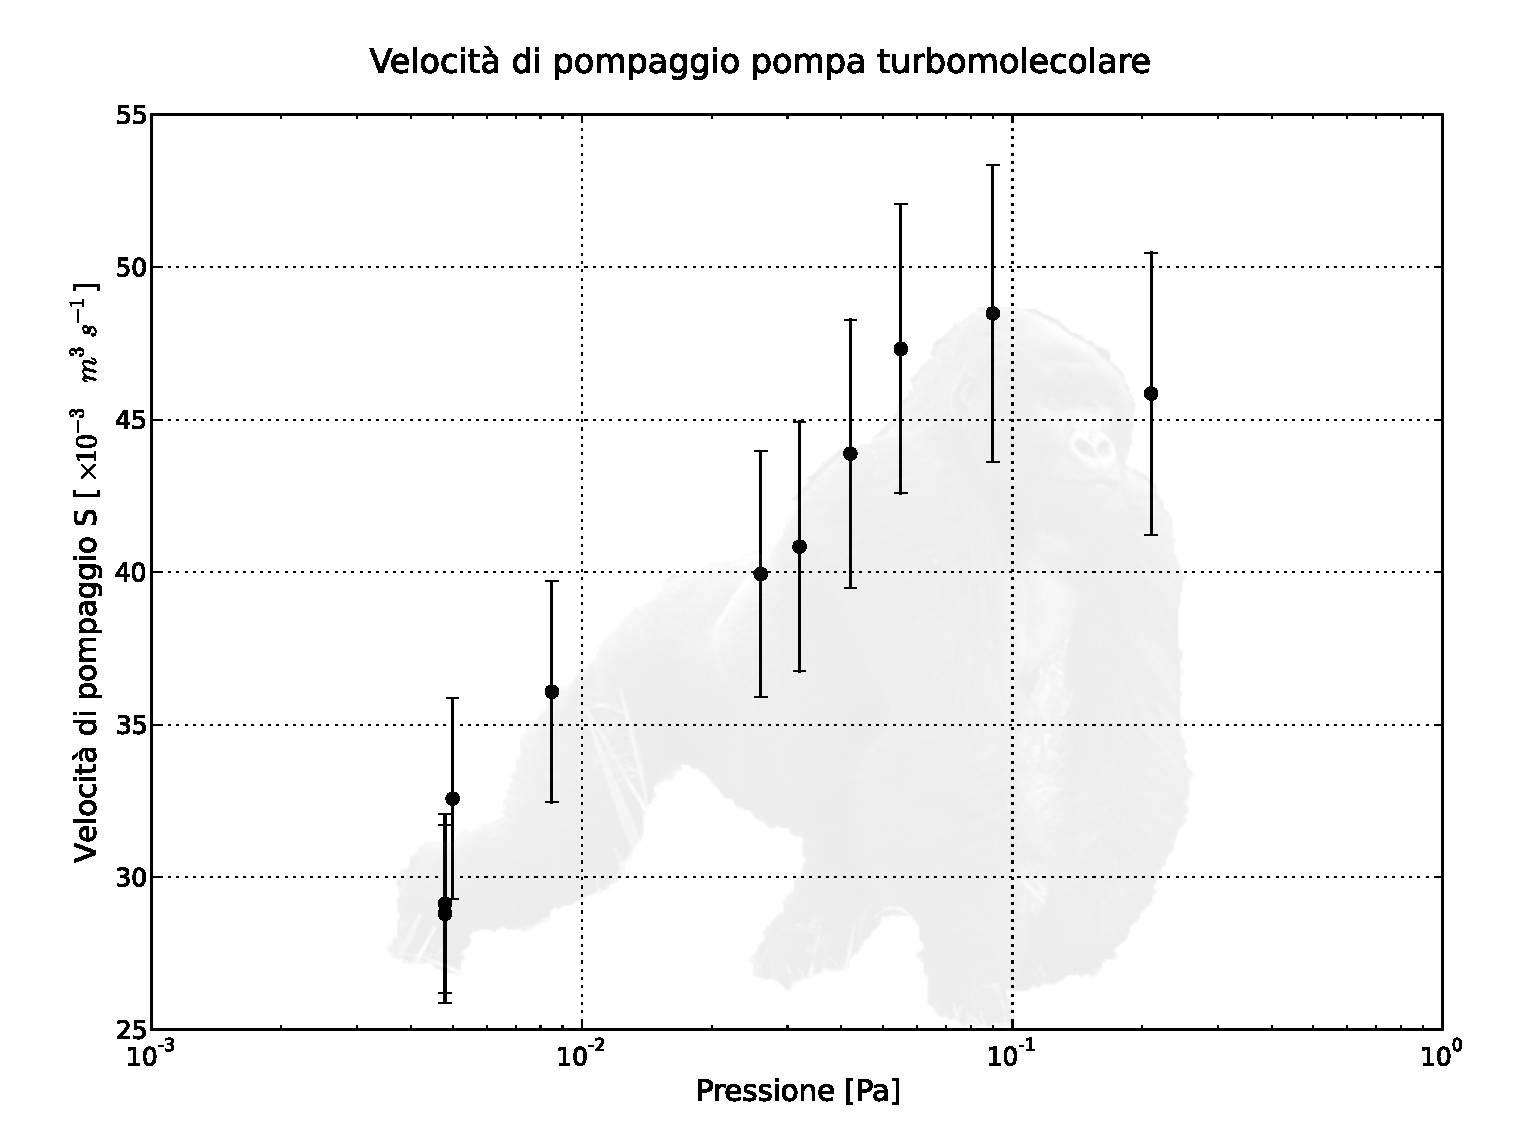
\includegraphics[width=14cm]{turbo.pdf}
		\label{fig:turbo}
	\caption{Il grafico mostra i valori elaborati della velocità di pompaggio della pompa turbomolecolare in funzione della pressione limite raggiunta in camera. L'asse delle ascisse ha scala logaritmica mentre l'asse delle ordinate ha scala lineare.}
\end{figure}